-% -*-coding: utf-8 -*-
%
% Tesis de virtualizacion
% Otubre 22 de 2014
%
% Original authors:
% William Adonis Diaz Valdez
% Carlos Ernesto Hernandez Granados
% Cesar Augusto Viana
%
% License:
% CC BY-NC-SA 3.0 (http://creativecommons.org/licenses/by-nc-sa/3.0/)
%
%
\begin{document}.
\documentclass{utec-thesis}
\pagenumbering{roman}

\university{\textbf{Universidad Tecnológica de El Salvador}}
\title{Análisis e interpretación de información de servidores seleccionados en la empresa Negocios Asociados S. A. para el estudio sobre la posibilidad de migración a un ambiente virtual utilizando tecnología Vmware en los nuevos servidores que serán adquiridos por la empresa con el fin de virtualizar.}

\authors{
  \begin{center}
    \begin{TAB}(r,700ex,3ex){ll}{cccc}
      \textbf{Integrantes} & \textbf{Carné}\\
      William Adonis Díaz Valdez & 25-5700-2008\\
      Carlos Ernesto Hernández Granados & 25-1242-2008\\
      Cesar Augusto Viana & 25-4407-2007\\
    \end{TAB}
  \end{center}
}


\begin{document}
\maketitle


% ----------------------------------------------------------------------------------------
%	LIST OF CONTENTS/FIGURES/TABLES PAGES
% ----------------------------------------------------------------------------------------

\begin{singlespace}
  \tableofcontents
\end{singlespace}

\cleardoublepage
\pagenumbering{arabic}

\chapter*{Introducción}
\addcontentsline{toc}{chapter}{Introducción}

Como aporte para la empresa Negocios Asociados S. A se ha desarrollado el presente trabajo con la finalidad de colaborar con el correcto desempeño de las labores cotidianas de los empleados que hacen uso de los sistemas de información y brindar apoyo que permita conocer las condiciones de funcionalidad de los servidores que brindan sus diferentes servicios para que los empleados puedan realizar sus labores cotidianas.

La empresa se dedica a comercializar productos eléctricos de baja, media y alta tensión, es una empresa regional que cuenta con muchas sucursales en la región Centroamericana, debido a esto tiene diseminado por la región muchos servidores con mucha información valiosa, pero nuestro trabajo se enfocara en una de las sucursales que se llama “Electrobodegas”, donde se encuentra centralizada mucha información y la mayoría del personal administrativo con que cuenta la empresa.

En la empresa se encuentran funcionando muchos servidores y algunos de ellos presentan algún tipo de dificultad y que expondremos a los miembros del equipo de IT de la empresa para que tomen en consideración nuestro estudio sobre los recursos con los que actualmente cuenta la empresa y que se tienen pensado llevarse a un ambiente virtual.

\chapter{Descripción del proyecto de investigación}

\section{Objetivos}

\subsection{Objetivo General}

Aportar a la empresa Negocios Asociados S. A. un análisis de los servidores que se podrían virtualizar, propuestos por la empresa, en el cual se estudiaran las características y especificaciones técnicas de cada uno y que arrojará los resultados para saber si estos pueden ser llevados a un ambiente virtual.


\subsection{Objetivos Específicos}

\begin{itemize}
\item Implementar herramientas de diagnóstico en los servidores escogidos que brinden la información necesaria para el análisis que arrojara los resultados necesarios para saber qué clase de equipos Negocios Asociados S. A. podría adquirir.

\item Diagnosticar y hacer observaciones sobre cualquier mal funcionamiento o irregularidad  que se encuentre durante el estudio de los equipos para posteriormente hacer recomendaciones sobre estos para así evitar futuras fallas que comprometan el funcionamiento de los servidores.

\item Presentar propuestas sobre la optimización de los recursos de los servidores que se van a convertir a máquinas virtuales para así aprovechar mejor los equipos tecnológicos que la empresa va adquirir.
\end{itemize}

\pagebreak

\section{Alcances y limitantes}

\subsection{Alcances}

\begin{itemize}
\item Recolectar la información necesaria sobre uso de recursos de entrada y salida de periféricos principales como memoria RAM, disco duros y procesador, así como uso de la red de los servidores que se podrían virtualizar.

\item Analizar el funcionamiento actual de los servidores y verificar posibles fallas que estos pudiesen tener como falta de recursos, aplicaciones ligadas a cierto software que el servidor utiliza o si hay un gran tráfico de red.

\item Crear una propuesta de hardware de los servidores que serán virtualizados para estos no sufran de falta de recursos o desperdicio de estos y que tecnología de virtualización les beneficiaría.
\end{itemize}

\subsection{Limitantes}

\begin{itemize}
\item Debe ser utilizada solo una herramientas de diagnostico para evitar que las herramientas de monitoreo gasten recursos en los servidores que se monitorearan.

\item Se enfoca en aquellas aplicaciones o servicios que tienen más importancia en los servidores.

\item Los recursos que serán recomendados serán aquellos que tienen
  mayor relevancia para la creación de una máquina virtual (memoria RAM, procesador, discos duros, tarjetas de red) en los servidores seleccionados por la empresa Negocios Asociados S.A.
\end{itemize}

\pagebreak

\section{Situación Problemática}

La situación en la empresa es la siguiente:

Como empresa han tomado la decisión de migrar algunos servidores a un ambiente virtualizado.

Algunas de las razones por la que se desean implementar virtualización son:

\begin{itemize}
\item Uno de los servidores ya no cuenta con fuente redundante
\item Problemas de espacio en almacenamiento
\item No tiene soporte en discos duros, esto por que ya no se encuentran discos para este modelo de servidor.
\item La información que se encuentra en el servidor es de vital importancia, ahí están las bases de datos de la empresa.
\item Uno de los servidor tiene problemas similares, en este funcionan el
  Active Directory, Servidor DHCP y servidor de aplicaciones.
\end{itemize}

\section{Justificación}
%{\let\clearpage\relax\section{Justificación}}

Muchas serian las ventajas que obtendría la empresa Negocios Asociados S. A. del proyecto que realizaremos.

\begin{itemize}
\item Conocimiento del rendimiento de sus servidores para la toma de decisiones.
\item Redimensionar el disco duro del servidor al momento de una posible migración a un ambiente virtual.
\item Optimizar el tamaño de la memoria ram para un mejor desempeño.
\item La empresa Negocios Asociados S.A obtendrá nuevo hardware para llevar acabo el proceso de migración.
\end{itemize}

\clearpage

\section{Cronograma de actividades}

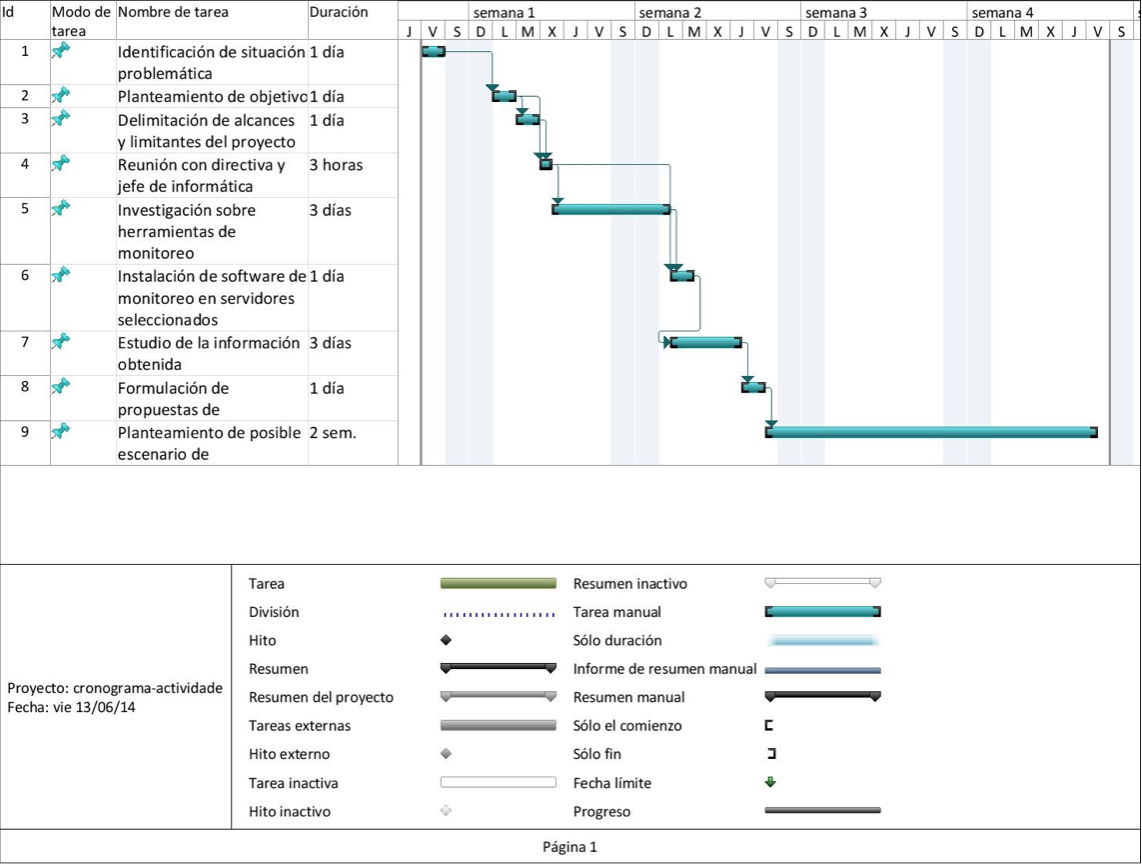
\includegraphics[width=\linewidth]{cronograma}

%\chapter{Marco te\'orico}

\section{Descripci\'on de la Empresa}

Grupo Electrobodegas pertenece a un grupo de empresas hermanas, que se dedican a comercializar productos eléctricos de baja, mediana y alta tension. Cuenta con un gran numero de clientes entre ellos personas, empresas, alcaldías, ONG’s, Gobierno Central, ademas compite en licitaciones para adjudicarse proyectos estatales de presupuesto mediano y grande.

\begin{center}
  Sitio web de Electro Bodegas: \url{http://www.electrobodegas.com/}

  \begin{figure}[h!]
    \centering
    
\includegraphics{electrobodegas}
    \caption{Logo de Electro Bodegas}
  \end{figure}
\end{center}

\\
\textbf{Ubicaci\'on:}

\begin{figure}
  \centering
  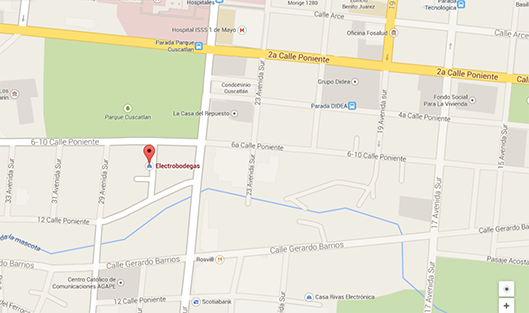
\includegraphics{electromap}
  \caption{Mapa de ubicación de Electro Bodegas (Vista satélite Google maps)}
\end{figure}

La empresa se encuentra en una ubicación accesible desde varios puntos de la capital, en la 27 av. Sur y $6\degree$ $10\degree$ calle poniente, al sur del parque Cuscatlan.

\textbf{Empresas hermanas:}

\begin{TAB}(r, 5pt, 1cm)[30pt]{cc}{cc}
  \vtop{
    \hbox{\strut 
\includegraphics[scale=0.3]{surtielectric}}
    \hbox{\strut \textbf{Surtielectric}}
    \hbox{\strut Ubicación: Av. España y}
    \hbox{Alameda Juan Pablo II los Próceres.}}
  &
  \vtop{
    \hbox{\strut 
\includegraphics[scale=0.3]{csh-logo}}
    \hbox{\strut \textbf{Csh Ingeniería}}
    \hbox{\strut Ubicación: Av. España y Alameda}
    \hbox{Juan Pablo II los Próceres.}}
  \\
  \vtop{
    \hbox{\strut 
\includegraphics[scale=0.3]{tecnelec}}
    \hbox{\strut \textbf{Tecnelec}}
    \hbox{\strut Ubicaci\'on: San Miguel.}}
  &
  \vtop{
    \hbox{\strut 
\includegraphics[scale=0.3]{pelsa-logo}}
    \hbox{\strut \textbf{Pelsa Panama}}}
  \\
\end{TAB}

%%% Local Variables:
%%% mode: latex
%%% TeX-master: "../virtualizacion"
%%% End:

\section{Descripción de las tecnologías, metodologías a utilizar
en el proyecto}

\subsection{Metodología a emplear}

Para realizar el monitoreo de los servidores se han tomado como
referencia dos programas de monitoreo de servidores las cuales fueron Nagios y Zenoss.

Nagios y Zenoss poseen características parecidas, al final del
estudio se decidió utilizar Zenoss como herramienta de monitoreo debido a experiencia
previa con este. A continuación listamos algunas

diferencias.

\subsection{Síntesis de las tecnologías a utilizar}

Una de las preguntas más comunes de los usuarios de software abierto
es la diferencia entre Zenoss y Nagios. Aunque Nagios tiene una de las
mayores bases instaladas de cualquier solución de monitoreo está
es una pregunta lógica pero Zenoss tiene una serie de características
que lo diferencian de Nagios. Nagios es básicamente un planificador
que ejecuta comprobaciones de mantenimiento y pruebas contra los
dispositivos de red y los reportes regresan los resultados. Nagios
también tienen una lista completa de extensiones o plugins que son
similar a los plugins de Zenoss. Así que es posible utilizar los
plugins de Nagios en Zenoss, ya que proporciona la capacidad de
ejecutarlos.

\begin{itemize}
\item \textbf{Descubrimiento automático} - Zenoss puede descubrir
  automáticamente hosts y iniciar a monitorizar de forma
  automática. Nagios requiere que se introduzca de forma manual en
  un archivo de configuración.
\item \textbf{Monitoreo de Rendimiento} - Zenoss puede generar gráficos de
  series de tiempo del rendimiento. Nagios no puede sin plugins
  adicionales o software. A menudo los usuarios utilizan el motor
  gráfico popular llamado Cacti, que aprovecha RRDTool para
  recopilar datos de series de tiempo.
\item \textbf{Gestión de Eventos} - Zenoss puede normalizar los
  datos dentro de eventos, más allá de la colección desde otra
  fuente y deduplicación los eventos almacenan las ocurrencias en un
  contador el cual permite a los usuarios configurar alertas basadas en
  la frecuencias de una alerta.
\item \textbf{Monitoreo de Logs del sistema} - Zenoss puede monitorear
  los registros del sistema Unix, Linux, Windows y más. En adición
  Zenoss puede ser utilizado para traducir los datos dentro de los
  evento y normalizarlos junto con la disponibilidad y rendimiento
  recopilados a través de otros métodos como SNMP y SSH.
\item \textbf{Alertas sofisticadas} - Las alertas de Nagios se pueden
  enviar a una dirección de correo electrónico o a un localizado
  basado en ciertas condiciones. Sin embargo, Zenoss tiene un sistema
  de alerta más robusto, donde las alertas pueden enviarse a una
  sola persona o a un grupo de individuos. El escalamiento de reglas
  puede hacerse cumplir de manera que cuando una alertas van sin
  reconocimiento, puedan ser promovidas a otro operador de red.
\end{itemize}

\subsubsection{Nagios}

Nagios es un sistema de monitorización de redes ampliamente utilizado, de código abierto, que vigila los equipos (hardware) y servicios (software) que se especifiquen, alertando cuando el comportamiento de los mismos no sea el deseado. Entre sus características principales figuran la monitorización de servicios de red (SMTP, POP3, HTTP, SNMP...), la monitorización de los recursos de sistemas hardware (carga del procesador, uso de los discos, memoria, estado de los puertos...), independencia de sistemas operativos, posibilidad de monitorización remota mediante túneles SSL cifrados o SSH, y la posibilidad de programar plugins específicos para nuevos sistemas.

Se trata de un software que proporciona una gran versatilidad para consultar prácticamente cualquier parámetro de interés de un sistema, y genera alertas, que pueden ser recibidas por los responsables correspondientes mediante (entre otros medios) correo electrónico y mensajes SMS, cuando estos parámetros exceden de los márgenes definidos por el administrador de red.

Llamado originalmente Netsaint, nombre que se debió cambiar por coincidencia con otra marca comercial, fue creado y es actualmente mantenido por Ethan Galstad, junto con un grupo de desarrolladores de software que mantienen también varios complementos.

Nagios fue originalmente diseñado para ser ejecutado en GNU/Linux, pero también se ejecuta bien en variantes de Unix.

Nagios está licenciado bajo la GNU General Public License Version 2
publicada por la Free Software Foundation.

\subsubsection{Características de Nagios}

\begin{itemize}
\item Monitorización de servicios de red (SMTP, POP3, HTTP, NNTP, ICMP, SNMP).
\item Monitorización de los recursos de equipos hardware (carga del procesador, uso de los discos, logs del sistema) en varios sistemas operativos, incluso Microsoft Windows con los plugins NRPE\_NT o \texttt{NSClient++}.
\item Monitorización remota, a través de túneles SSL cifrados o SSH.
\item Diseño simple de plugins, que permiten a los usuarios desarrollar sus propios chequeos de servicios dependiendo de sus necesidades, usando sus herramientas preferidas (Bash, \texttt{C++}, Perl, Ruby, Python, PHP, C\#$\ldots$).
\item Chequeo de servicios paralizados.
\item Posibilidad de definir la jerarquía de la red, permitiendo distinguir entre host caídos y host inaccesibles.
\item Notificaciones a los contactos cuando ocurren problemas en servicios o hosts, así como cuando son resueltos (a través del correo electrónico, busca personas, Jabber, SMS, o cualquier método definido por el usuario junto con su correspondiente complemento).
\item Posibilidad de definir manejadores de eventos que ejecuten al ocurrir un evento de un servicio o host para resoluciones de problemas proactivas.
\item Rotación automática del archivo de registro.
\item Soporte para implementar hosts de monitores redundantes.
\item Visualización del estado de la red en tiempo real a través de interfaz web, con la posibilidad de generar informes y gráficas de comportamiento de los sistemas monitorizados, y visualización del listado de notificaciones enviadas, historial de problemas, archivos de registros$\ldots$
\end{itemize}

\pagebreak

\subsubsection{Zenoss Core}

Zenoss Core es un software abierto, una plataforma de monitoreo de red
y sistema que es patrocinado por Zenoss, Inc. la cual desarrolla dos
versiones de Zenoss: Core y Enterprise. Core pertenece a la comunidad
y es desarrolla por la comunidad. \\
Zenoss Enterprise añade algunas características de valor sobre la
versión Core, tales como una librería extendida de reportes,
transacciones web sintéticas, monitores certificados (ZenPacks), y
un panel de administración para múltiples instalaciones de
Zenoss. Las características adicionales permiten a Zenoss
Inc. vender la versión Enterprise como un producto de software
comercial con soporte.

Zenoss Core es una solución de monitoreo que puede ser tan
completa como se desee. Y mientras que casi cualquier
persona puede instalarlo, correrlo, y monitorear un equipo, Zenoss Core
se torna un poco complicado en ocasiones. La
interfaz ha mejorado drásticamente en la versión 2, pero no es el
tipo de software que se puede utilizar de forma intuitiva, un poco de
orientación es necesaria.

Zenoss Core provee una solución de monitoreo que incorpora los
siguiente:
\begin{itemize}
\item Gestión de dispositivos
\item Monitoreo de disponibilidad
\item Gráficos de rendimiento
\item Gestión de usuarios y alertas
\item Arquitectura de plugins
\item Informes de seguimiento
\end{itemize}

Para monitorear activos de Tecnología de información (Servidores,
routers, switches, sitios web, y cualquier cosa conectada a la red),
se debe instalar Zenoss Core en un servidor. A pesar que Zenoss Core
está diseñado para ser instalado en un servidor Linux,
aplicaciones virtuales están disponibles para permitir a los
usuarios de Machintosh y Windows instalar Zenoss core utilizando
VMware.

Después de la instalación, usted puede manejar su instalación de
Zenoss Core y su configuración de monitorización de una interfaz
web. La siguiente imagen muestra la vista del panel: \\

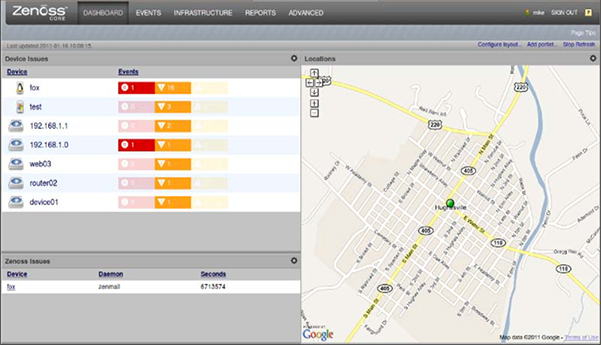
\includegraphics[width=\linewidth]{zenoss-dashboard}

El portal web es la cara del sistema de Zenoss Core y es el lugar
donde pasamos la mayor parte de nuestro tiempo. Este provee un único
acceso para el sistema de monitoreo y no requiere saber acerca del
sistema operativo. La interfaz web ofrecer arrastrar y soltar,
portlets que muestra una vista personalizada de la red en cualquier
punto.

\subsubsection{Gestión de dispositivos}

En el corazón de la gestión de dispositivos, Zenoss Core utiliza
una Base de Datos de la Gestión de Configuración (CMDB), el cual
almacena un modelo del entorno de TI a la CMDB de una en una o por
auto-descubrimiento de dispositivos activos al recorrer la tabla de
enrutamiento. Los dispositivos son gestionados a través  de
protocolo simple de administración de red (SNMP), SSH (o Telnet), o
escaneos de puertos.

Zenoss Core permite organizar dispositivos por ubicaciones definidas
por el usuario, grupos y sistemas. Uno de los más poderosos
conceptos organizativos de Zenoss Core es clases, el cual permite
definir las características de monitoreo basadas en una
clasificación jerárquica de los dispositivos, lo que permite a un
dispositivo a heredar las propiedades de seguimiento de su clase padre.

La siguiente captura de pantalla ofrece un vistazo a una página de
estado del dispositivo: \\

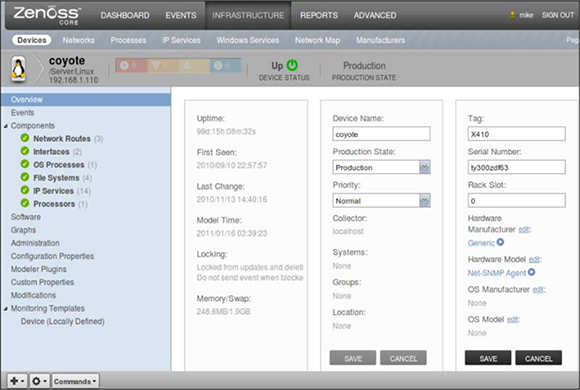
\includegraphics[width=\linewidth]{zenoss-dmanagement}

\subsubsection{Monitores de disponibilidad y rendimiento}

Mediante el uso de la motorización ICMP y SNMP, Zenoss Core informa
sobre la disponibilidad de los siguiente:

\begin{itemize}
\item Dispositivos de red
\item Servicios y puerto TCP/IP
\item Disponibilidad de URL
\item Servicios y procesos de Windows
\item Procesos de Linux\textbackslash{}UNIX
\end{itemize}

Zenoss Core está en el nivel 3 de la topología de red, lo cual
reduce la cantidad de alertas mediante la creación de un evento
solamente sobre el dispositivo problemático y no sobre los dispositivos
que dependen de el.

Monitores de rendimiento recopilan datos de series de tiempo y son
proporcionados con un análisis gráfico de los siguientes
componentes:

\begin{itemize}
\item Estadísticas del sistema de ficheros.
\item Uso de CPU y memoria.
\item Monitoreo de JMX para servidores J2EE (disponible a través de
  un ZenPack).
\item Soporte para plugins Nagios y Cacti.
\end{itemize}

La siguiente imagen muestra un gráfico basado en la
actividad de monitoreo de Zenoss Core: \\

\centerline{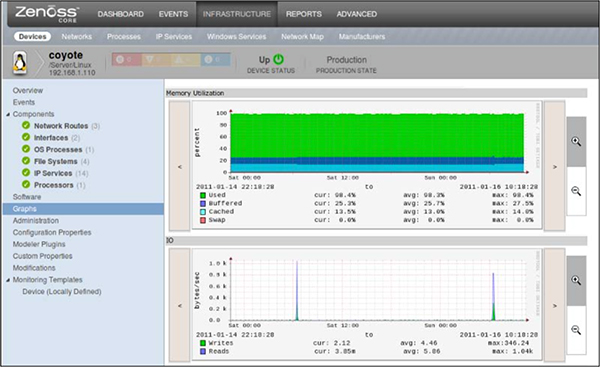
\includegraphics[scale=0.71]{zenoss-performance}}

Utilizando el sistema de gestión de eventos incorporado, se puede
configurar Zenoss Core para generar un evento si un dispositivo
supervisado cruza un umbral definido.

\subsubsection{Gestión de eventos}

Zenoss Core monitorea una variedad de recursos en busca de problemas,
incluyendo logs del sistema, disponibilidad y monitoreo de
rendimiento, trampas SNMP, registros de eventos de Windows y scripts
personalizados. Las características principales del sistema de
gestión de eventos incluyen:

\begin{itemize}
\item Eventos personalizados
\item Priorización automática de eventos
\item Duplicación de eventos
\item Correlación de eventos Arriba$\backslash$Abajo
\end{itemize}

La siguiente imagen muestra la \textbf{Consola de
  Eventos:} \\

\centerline{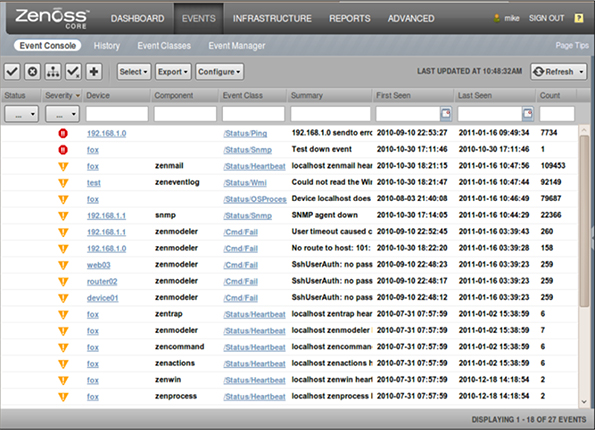
\includegraphics[scale=0.71]{zenoss-events}}

El sistema de ventos mitiga eventos duplicados y borra automaticamente
eventos cuando el estado de los eventos cambia de inactivo a
activo. Zenoss Core también recopilar eventos de secuencias de
comandos personalizadas y aplicaciones externas.
En respuesta a los acontecimientos, Zenoss Core puede enviar correo
electrónicos o paginas de alertas, correr un script o no hacer
nada. Zenoss Core puede ser configurado para responder a un evento
mediante la definición de reglas de alerta. Las reglas de alertas
son definidas en base aun usuario o grupo de usuarios.

\pagebreak

\subsubsection{Arquitectura de plugins}

Zenoss Core ofrece varias maneras para extender la funcionalidad base:

\begin{itemize}
\item ZenPacks: Zenoss Core complemento de módulos
\item Plugins de Nagios
\item Plugins de Cacti
\end{itemize}

La arquitectura ZenPack permite empaquetar plugins y configuraciones
para su distribución a otros usuario y la comunidad en general.

\subsubsection{Reportes del sistema}

Zenoss Corre contiene un conjunto de reportes estándar que permiten
ver que está sucediendo en este momento, así como lo que ha
sucedido en el pasado. Los informes se integran con la gestión de
dispositivos, monitores de rendimiento, eventos y funcionalidades de
usuario.

La siguiente imagen muestra el reporte de Todos los
componentes monitoreados: \\

\centerline{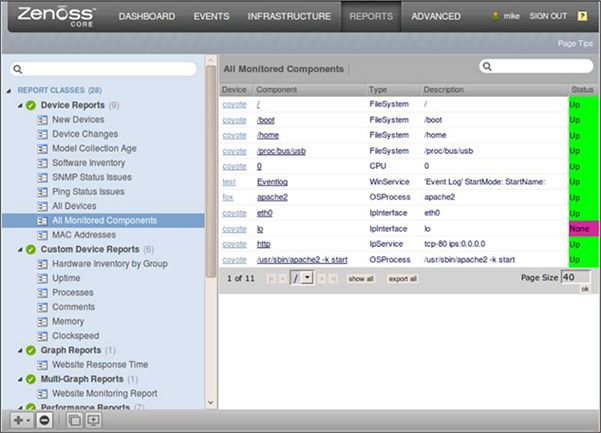
\includegraphics[scale=0.35]{zenoss-reports}}

\subsubsection{Informes personalizados de dispositivos}

Zenoss Core permite a los usuarios escribir informes personalizados de
dispositivos en la interfaz web, como se ven en la siguiente captura
de pantalla: \\

\centerline{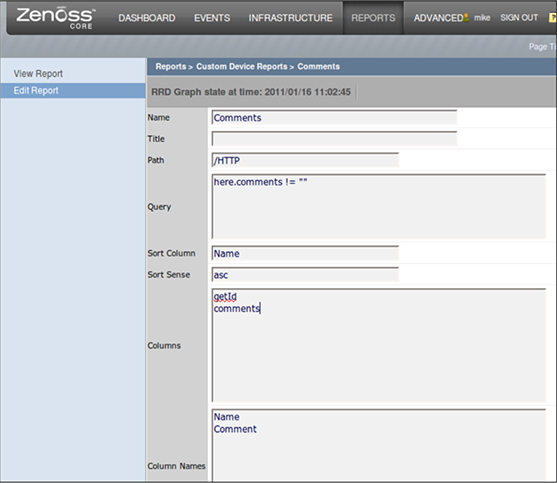
\includegraphics[scale=0.71]{zenoss-devices}}

\clearpage

\subsection{Cuadros comparativos}

\begin{TAB}(r,5pt,5pt)[9pt]{|l|c|c|}{|c|c|c|c|c|c|c|c|c|c|c|c|c|c|c|c|c|c|}% (rows,min,max)[tabcolsep]{columns}{rows}
\textbf{Nombre}                     & Nagios & Zenoss \\
\textbf{Gráficas}                   & Si     & Si     \\
\textbf{Informes SLA}               & Si     & No     \\
\textbf{Grupos Lógicos}             & Si     & Si     \\
\textbf{Estadísticas}               & Si     & Si     \\
\textbf{Predicción de estadísticas} & Si     & Si     \\
\textbf{Autodescubrimiento}         & Si     & Si     \\
\textbf{Agentes}                    & Si     & SNMP, WMI, IMX, etc. \\
\textbf{SNMP}                       & A través de plugin & Si     \\
\textbf{Syslog}                     & Si     & Si     \\
\textbf{Scripts externos}           & Si     & Si     \\
\textbf{Complementos (plugins)}     & Si     & Si     \\
\textbf{Creación de complementos} & Media  & Fácil \\
\textbf{Alertas}                    & Si     & Si      \\
\textbf{Aplicación web}           & Solo virtualización & Control total \\
\textbf{Monitorización distribuida} & Si & Si \\
\textbf{Método de almacenaje de datos} & SQL & RRDtool y MySQL \\
\textbf{Licencia}                   & GPL    & GPL      \\
\end{TAB}

%%% Local Variables:
%%% mode: latex
%%% TeX-master: "../virtualizacion"
%%% End:


\end{document}
